
\chapter{Another Appendix Chapter}
\label{chap:A2}

\subsection{Client Library Used for Experiments in Subsection~\ref{cha:testing:onedevice}} \label{chap:A2:onedeviceclientlib}
\begin{lstlisting}[language=Rust, style=boxed, showstringspaces=false]{}
use std::error::Error;

use NOSHP_Client::{
    client::{ClientState, NoshpClient, 
        Request, UserDefinedState},
    client_config::{ClientConfig, ParsedConfig},
};

#[derive(Default)]
struct ExampleState {
    text: String,
}
impl UserDefinedState for ExampleState {}

const CONFIG_PATH: &str = "./example_config.toml";
#[tokio::main]
async fn main() -> Result<(), Box<dyn Error>> {
    let config = ClientConfig::load_config(CONFIG_PATH);
    let config = match config {
        Ok(r) => r,
        Err(e) => {
            eprintln!(
                "Error loading config: {}", e.to_string()
            );
            println!("Loading default config...");
            ParsedConfig::default()
        }
    };

    let client_handler = NoshpClient::new();
    client_handler
        .set_state(ExampleState {
            text: String::from("hello world"),
        })
        .add_callback("Turn On", Box::new(turn_on_led))
        .add_callback("Turn Off", Box::new(turn_off_led))
        .run(config)
        .await
        .unwrap();

    return Ok(());
}

fn turn_on_led(
    _state: &mut ClientState<ExampleState>,
    _req: Request
) {
    println!("Turn On")
}

fn turn_off_led(
    _state: &mut ClientState<ExampleState>,
    _req: Request
) {
    println!("Turn Off")
}
\end{lstlisting}


\subsection{OS Error encountered during client spawning} 
Error when attempting to spawn 1000 clients.
\label{chap:A2:oserror}
\begin{figure}[h]
\caption{Linux TCP Error}
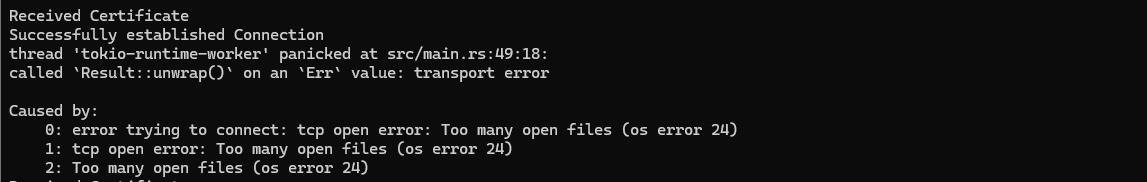
\includegraphics[width=\textwidth]{os_error_tcp_new.png}
\label{fig:tcperror}
\end{figure}
